\pdfoutput=1

\documentclass[10pt,letterpaper]{article}

\usepackage[utf8]{inputenc} % allow utf-8 input
\usepackage[T1]{fontenc}    % use 8-bit T1 fonts
\usepackage{lmodern}
\usepackage{hyperref}       % hyperlinks
\usepackage{url}            % simple URL typesetting
\usepackage{booktabs}       % professional-quality tables
\usepackage{amsfonts}       % blackboard math symbols
\usepackage{nicefrac}       % compact symbols for 1/2, etc.
\usepackage{microtype}      % microtypography
\usepackage{xspace}
\usepackage{authblk}

\usepackage{graphicx}
\graphicspath{{pictures/}}
\usepackage{amsmath}
\usepackage{amssymb}
\usepackage{amsthm}
\usepackage{bm}
\usepackage[margin=1in]{geometry}

\usepackage[font=small]{caption}
\usepackage{subcaption}
\usepackage{tikz}
\usepackage{pgfplots}
\usepackage{fp}
\usetikzlibrary{bayesnet}

\theoremstyle{plain}
\newtheorem{thm}{Theorem}[section]
\newtheorem{lem}[thm]{Lemma}
\newtheorem{prop}[thm]{Proposition}
\newtheorem*{cor}{Corollary}

\theoremstyle{definition}
\newtheorem{defn}{Definition}[section]
\newtheorem{conj}{Conjecture}[section]
\newtheorem{exmp}{Example}[section]

\theoremstyle{remark}
\newtheorem*{rem}{Remark}
\newtheorem*{note}{Note}

\DeclareMathOperator*{\argmin}{arg\,min}
\newcommand{\normk}[1] {\left\| #1 \right\|_k}
\newcommand{\norm}[1] {\left\| #1 \right\|}
\newcommand{\abs}[1] {| #1 |}
\newcommand{\normtwo}[1] {\left\| #1 \right\|_2}
\newcommand{\normf}[1] {\left\| #1 \right\|_{\mathcal{F}}}
\newcommand{\frob}[1]{\|#1\|_\mathcal{F}}
\newcommand{\sumz}{\sum_{z=1}^Z}
\newcommand{\sumi}{\sum_{i=1}^m}
\newcommand{\sump}{\sum_{p=1}^L}
\newcommand{\sumiz}[1]{\sum_{#1=1 | z_{#1}=z}^m}
\newcommand{\sumik}[1]{\sum_{#1=1 | k_{#1}=k}^m}
\newcommand{\sumk}{\sum_{k=1}^L}
\newcommand{\mul}[1] {{\mu}_{\mkern-0.66\thinmuskip\mathcal{L}} (#1) }

\newcommand{\wrt}{w.r.t.\@\xspace}

\newcommand\todo[1]{\textcolor{red}{#1}}
\renewcommand\todo[1]{}

\newcommand{\twocol}[2]{
    \begin{tabular}{cc}
        #1 & #2 
    \end{tabular}
}

\newcommand{\landSVM}{L$^3$-SVMs\xspace}

\author[1]{Zantedeschi Valentina \\
\href{mailto:valentina.zantedeschi@univ-st-etienne.fr}{valentina.zantedeschi@univ-st-etienne.fr}}
\author[1]{\\Emonet R\'emi\\
\href{mailto:remi.emonet@univ-st-etienne.fr}{remi.emonet@univ-st-etienne.fr}}
\author[1]{\\Sebban Marc\\
\href{mailto:marc.sebban@univ-st-etienne.fr}{marc.sebban@univ-st-etienne.fr}}

\affil[1]{
Univ Lyon, UJM-Saint-Etienne, CNRS, Institut d Optique Graduate School, Laboratoire Hubert Curien UMR 5516, F-42023, SAINT-ETIENNE, France
}

\title{\landSVM: \\Landmarks-based Linear Local Support Vector Machines}
\date{}

\begin{document}

\maketitle


\begin{abstract}
For their ability to capture non-linearities in the data and to scale to large training sets, local Support Vector Machines (SVMs) have received a special attention during the past decade. 
In this paper, we introduce a new local SVM method, called \landSVM, which clusters the input space, carries out dimensionality reduction by projecting the data on landmarks, and jointly learns a linear combination of local  models. Simple and effective, our algorithm is also theoretically well-founded. Using the framework of Uniform Stability, we show that our SVM formulation comes with generalization guarantees on the true risk. 
The experiments based on the simplest configuration of our model (i.e. landmarks randomly selected, linear projection, linear kernel) show that \landSVM is very competitive \wrt the state of the art and opens the door to new exciting  lines of research.
\end{abstract}
% !TEX root = ../arxiv.tex

Unsupervised domain adaptation (UDA) is a variant of semi-supervised learning \cite{blum1998combining}, where the available unlabelled data comes from a different distribution than the annotated dataset \cite{Ben-DavidBCP06}.
A case in point is to exploit synthetic data, where annotation is more accessible compared to the costly labelling of real-world images \cite{RichterVRK16,RosSMVL16}.
Along with some success in addressing UDA for semantic segmentation \cite{TsaiHSS0C18,VuJBCP19,0001S20,ZouYKW18}, the developed methods are growing increasingly sophisticated and often combine style transfer networks, adversarial training or network ensembles \cite{KimB20a,LiYV19,TsaiSSC19,Yang_2020_ECCV}.
This increase in model complexity impedes reproducibility, potentially slowing further progress.

In this work, we propose a UDA framework reaching state-of-the-art segmentation accuracy (measured by the Intersection-over-Union, IoU) without incurring substantial training efforts.
Toward this goal, we adopt a simple semi-supervised approach, \emph{self-training} \cite{ChenWB11,lee2013pseudo,ZouYKW18}, used in recent works only in conjunction with adversarial training or network ensembles \cite{ChoiKK19,KimB20a,Mei_2020_ECCV,Wang_2020_ECCV,0001S20,Zheng_2020_IJCV,ZhengY20}.
By contrast, we use self-training \emph{standalone}.
Compared to previous self-training methods \cite{ChenLCCCZAS20,Li_2020_ECCV,subhani2020learning,ZouYKW18,ZouYLKW19}, our approach also sidesteps the inconvenience of multiple training rounds, as they often require expert intervention between consecutive rounds.
We train our model using co-evolving pseudo labels end-to-end without such need.

\begin{figure}[t]%
    \centering
    \def\svgwidth{\linewidth}
    \input{figures/preview/bars.pdf_tex}
    \caption{\textbf{Results preview.} Unlike much recent work that combines multiple training paradigms, such as adversarial training and style transfer, our approach retains the modest single-round training complexity of self-training, yet improves the state of the art for adapting semantic segmentation by a significant margin.}
    \label{fig:preview}
\end{figure}

Our method leverages the ubiquitous \emph{data augmentation} techniques from fully supervised learning \cite{deeplabv3plus2018,ZhaoSQWJ17}: photometric jitter, flipping and multi-scale cropping.
We enforce \emph{consistency} of the semantic maps produced by the model across these image perturbations.
The following assumption formalises the key premise:

\myparagraph{Assumption 1.}
Let $f: \mathcal{I} \rightarrow \mathcal{M}$ represent a pixelwise mapping from images $\mathcal{I}$ to semantic output $\mathcal{M}$.
Denote $\rho_{\bm{\epsilon}}: \mathcal{I} \rightarrow \mathcal{I}$ a photometric image transform and, similarly, $\tau_{\bm{\epsilon}'}: \mathcal{I} \rightarrow \mathcal{I}$ a spatial similarity transformation, where $\bm{\epsilon},\bm{\epsilon}'\sim p(\cdot)$ are control variables following some pre-defined density (\eg, $p \equiv \mathcal{N}(0, 1)$).
Then, for any image $I \in \mathcal{I}$, $f$ is \emph{invariant} under $\rho_{\bm{\epsilon}}$ and \emph{equivariant} under $\tau_{\bm{\epsilon}'}$, \ie~$f(\rho_{\bm{\epsilon}}(I)) = f(I)$ and $f(\tau_{\bm{\epsilon}'}(I)) = \tau_{\bm{\epsilon}'}(f(I))$.

\smallskip
\noindent Next, we introduce a training framework using a \emph{momentum network} -- a slowly advancing copy of the original model.
The momentum network provides stable, yet recent targets for model updates, as opposed to the fixed supervision in model distillation \cite{Chen0G18,Zheng_2020_IJCV,ZhengY20}.
We also re-visit the problem of long-tail recognition in the context of generating pseudo labels for self-supervision.
In particular, we maintain an \emph{exponentially moving class prior} used to discount the confidence thresholds for those classes with few samples and increase their relative contribution to the training loss.
Our framework is simple to train, adds moderate computational overhead compared to a fully supervised setup, yet sets a new state of the art on established benchmarks (\cf \cref{fig:preview}).










\section{Proposed Approach} \label{sec:method}

Our goal is to create a unified model that maps task representations (e.g., obtained using task2vec~\cite{achille2019task2vec}) to simulation parameters, which are in turn used to render synthetic pre-training datasets for not only tasks that are seen during training, but also novel tasks.
This is a challenging problem, as the number of possible simulation parameter configurations is combinatorially large, making a brute-force approach infeasible when the number of parameters grows. 

\subsection{Overview} 

\cref{fig:controller-approach} shows an overview of our approach. During training, a batch of ``seen'' tasks is provided as input. Their task2vec vector representations are fed as input to \ours, which is a parametric model (shared across all tasks) mapping these downstream task2vecs to simulation parameters, such as lighting direction, amount of blur, background variability, etc.  These parameters are then used by a data generator (in our implementation, built using the Three-D-World platform~\cite{gan2020threedworld}) to generate a dataset of synthetic images. A classifier model then gets pre-trained on these synthetic images, and the backbone is subsequently used for evaluation on specific downstream task. The classifier's accuracy on this task is used as a reward to update \ours's parameters. 
Once trained, \ours can also be used to efficiently predict simulation parameters in {\em one-shot} for ``unseen'' tasks that it has not encountered during training. 


\subsection{\ours Model} 


Let us denote \ours's parameters with $\theta$. Given the task2vec representation of a downstream task $\bs{x} \in \mc{X}$ as input, \ours outputs simulation parameters $a \in \Omega$. The model consists of $M$ output heads, one for each simulation parameter. In the following discussion, just as in our experiments, each simulation parameter is discretized to a few levels to limit the space of possible outputs. Each head outputs a categorical distribution $\pi_i(\bs{x}, \theta) \in \Delta^{k_i}$, where $k_i$ is the number of discrete values for parameter $i \in [M]$, and $\Delta^{k_i}$, a standard $k_i$-simplex. The set of argmax outputs $\nu(\bs{x}, \theta) = \{\nu_i | \nu_i = \argmax_{j \in [k_i]} \pi_{i, j} ~\forall i \in [M]\}$ is the set of simulation parameter values used for synthetic data generation. Subsequently, we drop annotating the dependence of $\pi$ and $\nu$ on $\theta$ and $\bs{x}$ when clear.

\subsection{\ours Training} 


Since Task2Sim aims to maximize downstream accuracy after pre-training, we use this accuracy as the reward in our training optimization\footnote{Note that our rewards depend only on the task2vec input and the output action and do not involve any states, and thus our problem can be considered similar to a stateless-RL or contextual bandits problem \cite{langford2007epoch}.}.
Note that this downstream accuracy is a non-differentiable function of the output simulation parameters (assuming any simulation engine can be used as a black box) and hence direct gradient-based optimization cannot be used to train \ours. Instead, we use REINFORCE~\cite{williams1992simple}, to approximate gradients of downstream task performance with respect to model parameters $\theta$. 

\ours's outputs represent a distribution over ``actions'' corresponding to different values of the set of $M$ simulation parameters. $P(a) = \prod_{i \in [M]} \pi_i(a_i)$ is the probability of picking action $a = [a_i]_{i \in [M]}$, under policy $\pi = [\pi_i]_{i \in [M]}$. Remember that the output $\pi$ is a function of the parameters $\theta$ and the task representation $\bs{x}$. To train the model, we maximize the expected reward under its policy, defined as
\begin{align}
    R = \E_{a \in \Omega}[R(a)] = \sum_{a \in \Omega} P(a) R(a)
\end{align}
where $\Omega$ is the space of all outputs $a$ and $R(a)$ is the reward when parameter values corresponding to action $a$ are chosen. Since reward is the downstream accuracy, $R(a) \in [0, 100]$.  
Using the REINFORCE rule, we have
\begin{align}
    \nabla_{\theta} R 
    &= \E_{a \in \Omega} \left[ (\nabla_{\theta} \log P(a)) R(a) \right] \\
    &= \E_{a \in \Omega} \left[ \left(\sum_{i \in [M]} \nabla_{\theta} \log \pi_i(a_i) \right) R(a) \right]
\end{align}
where the 2nd step comes from linearity of the derivative. In practice, we use a point estimate of the above expectation at a sample $a \sim (\pi + \epsilon)$ ($\epsilon$ being some exploration noise added to the Task2Sim output distribution) with a self-critical baseline following \cite{rennie2017self}:
\begin{align} \label{eq:grad-pt-est}
    \nabla_{\theta} R \approx \left(\sum_{i \in [M]} \nabla_{\theta} \log \pi_i(a_i) \right) \left( R(a) - R(\nu) \right) 
\end{align}
where, as a reminder $\nu$ is the set of the distribution argmax parameter values from the \name{} model heads.

A pseudo-code of our approach is shown in \cref{alg:train}.  Specifically, we update the model parameters $\theta$ using minibatches of tasks sampled from a set of ``seen'' tasks. Similar to \cite{oh2018self}, we also employ self-imitation learning biased towards actions found to have better rewards. This is done by keeping track of the best action encountered in the learning process and using it for additional updates to the model, besides the ones in \cref{ln:update} of \cref{alg:train}. 
Furthermore, we use the test accuracy of a 5-nearest neighbors classifier operating on features generated by the pretrained backbone as a proxy for downstream task performance since it is computationally much faster than other common evaluation criteria used in transfer learning, e.g., linear probing or full-network finetuning. Our experiments demonstrate that this proxy evaluation measure indeed correlates with, and thus, helps in final downstream performance with linear probing or full-network finetuning. 






\begin{algorithm}
\DontPrintSemicolon
 \textbf{Input:} Set of $N$ ``seen'' downstream tasks represented by task2vecs $\mc{T} = \{\bs{x}_i | i \in [N]\}$. \\
 Given initial Task2Sim parameters $\theta_0$ and initial noise level $\epsilon_0$\\
 Initialize $a_{max}^{(i)} | i \in [N]$ the maximum reward action for each seen task \\
 \For{$t \in [T]$}{
 Set noise level $\epsilon = \frac{\epsilon_0}{t} $ \\
 Sample minibatch $\tau$ of size $n$ from $\mc{T}$  \\
 Get \ours output distributions $\pi^{(i)} | i \in [n]$ \\
 Sample outputs $a^{(i)} \sim \pi^{(i)} + \epsilon$ \\
 Get Rewards $R(a^{(i)})$ by generating a synthetic dataset with parameters $a^{(i)}$, pre-training a backbone on it, and getting the 5-NN downstream accuracy using this backbone \\
 Update $a_{max}^{(i)}$ if $R(a^{(i)}) > R(a_{max}^{(i)})$ \\
 Get point estimates of reward gradients $dr^{(i)}$ for each task in minibatch using \cref{eq:grad-pt-est} \\
 $\theta_{t,0} \leftarrow \theta_{t-1} + \frac{\sum_{i \in [n]} dr^{(i)}}{n}$ \label{ln:update} \\
 \For{$j \in [T_{si}]$}{ 
    \tcp{Self Imitation}
    Get reward gradient estimates $dr_{si}^{(i)}$ from \cref{eq:grad-pt-est} for $a \leftarrow a_{max}^{(i)}$ \\
    $\theta_{t, j}  \leftarrow \theta_{t, j-1} + \frac{\sum_{i \in [n]} dr_{si}^{(i)}}{n}$
 }
 $\theta_{t} \leftarrow \theta_{t, T_{si}}$
 }
 \textbf{Output}: Trained model with parameters $\theta_T$. 
 \caption{Training Task2Sim}
 \label{alg:train}  
\end{algorithm}

\begin{table}[!b]
\centering
\caption{
\footnotesize
The correlation of our proposed pointwise evaluation metric \proposed~with the standard listwise metrics - Pearson's $r$, Spearman's $\rho$, Kendall's $\tau$ and sARE. The rank correlations between each pair of QPP system ranks (evaluated with a listwise measure and a pointwise measure) were computed with Kendall's $\tau$.
The high values indicate that the pointwise measurement can effectively \textit{substitute} a standard list-based measure, since they lead to a fairly similar relative ordering between the effectiveness of different QPP methods.
% measured via Pearson's, Spearman's, and Kendall's )between
% the relative ranked list of 7 QPP systems obtained by the standard listwise QPP evaluation approach ($r, \rho, \tau$) and our proposed pointwise models, $\pwu$ (left group) and $\pws$ (right group). For pointwise models, predicted QPP scores for individual queries are aggregated to compute the overall QPP system's score.
}
% \vskip 0.3em
\begin{adjustbox}{width=0.75\columnwidth}
% \begin{tabular}[c]{bssssss}
%\begin{tabular}{@{}lcccccc@{}}
\begin{tabular}{@{}l@{~~}c@{~~}c@{~~}c@{~~}c@{~~~~}c@{~~}c@{~~}c@{~~}c@{~~~~}c@{~~}c@{~~}c@{~~}c@{}}
\toprule
&\multicolumn{4}{c}{ $\pwua{\text{avg}}$}
&\multicolumn{4}{c}{ $\pwua{\text{min}}$}
&\multicolumn{4}{c}{ $\pwua{\text{max}}$}
\\

\cmidrule(r){2-5}
\cmidrule(r){6-9}
\cmidrule(r){10-13}

& \multicolumn{1}{c}{$r$} 
& \multicolumn{1}{c}{$\rho$} 
& \multicolumn{1}{c}{$\tau$}
& \multicolumn{1}{c}{$\text{sARE}$}
& \multicolumn{1}{c}{$r$} 
& \multicolumn{1}{c}{$\rho$} 
& \multicolumn{1}{c}{$\tau$}
& \multicolumn{1}{c}{$\text{sARE}$}
& \multicolumn{1}{c}{$r$} 
& \multicolumn{1}{c}{$\rho$} 
& \multicolumn{1}{c}{$\tau$}
& \multicolumn{1}{c}{$\text{sARE}$}
\\

\midrule
BM25 
& 0.810 & 0.810 & 0.905 & 0.887 
& 0.778 & 0.778 & 0.794 & 0.813 
& 0.802 & 0.810 & 0.794 & 0.794 \\

LMDir\;\;\;
& \textbf{0.905} & \textbf{0.810} & \textbf{0.905} & \textbf{0.887} 
& 0.778 & 0.794 & 0.794 & 0.810 
& 0.769 & 0.782 & 0.794 & 0.796 \\

LMJM 
& 0.810 & 0.810 & 0.810 & 0.846 
& 0.794 & 0.794 & 0.782 & 0.786 
& 0.794 & 0.769 & 0.810 & 0.846 \\
\bottomrule
\end{tabular}
\end{adjustbox}
\label{tab:stable}
\end{table}
\section{Numerical experiments}
\label{sec:expe}

We test the performance of the exact/inexact IPG algorithm for our product-space data driven CS reconstruction using the four datasets described in Table \ref{tab:data}. The datasets are uniformly sampled (populated) from 2-dimensional continuous manifolds embedded in a higher ambient dimension, see also  Figure~\ref{fig:datasets}\footnote{The S-manifold, Swiss roll and Oscillating wave are synthetic machine learning  datasets available e.g. in \cite{GMRA12}. The Magnetic Resonance Fingerprints (MRF) is generated by solving the Bloch dynamic equation for a uniform grid of relaxation times $T1,T2$ and for an external magnetic excitation pattern, discussed and implemented in~\cite{MRF}.}. 

To proceed with fast ANN searches within IPG, we separately build a cover tree structure per dataset i.e. a preprocessing step. As illustrated for the MRF manifold in Figure~\ref{fig:CT} the coverage levels 
%(highlighted in colours for segments associated with tree nodes at certain scale) 
decrease in a coarse-to-fine manner as we traverse down the tree i.e. increasing the scale.

%============TABLE DATA=========================
\ifCLASSOPTIONtwocolumn
\begin{table}[t!]
	\centering
	\scalebox{.91}{
	\begin{tabular}{ccccc}
		%\hline
		\toprule[.2em]
		Dataset & Population ($d$) & Ambient dim. ($\n$)&CT depth&CT res.\\
		\midrule[.1em]
		S-Manifold & 5000 & 200& 14&2.43E-4 \\
		%\hline
		Swiss roll & 5000 & 200 &14&1.70E-4\\
		%\hline
		Oscillating wave & 5000 & 200 &14&1.86E-4\\
		%\hline
		MR Fingerprints & 29760 & 512& 13&3.44E-4\\
		%\hline
		\bottomrule[.2em]
	\end{tabular}}
	\caption{Datasets for data-driven CS evaluations; a cover tree (CT) structure is formed for each dataset. The last two columns respectively report the number of scales and the finest covering resolution of each tree.  }
	\label{tab:data}	
\end{table}
\else
\begin{table}[t!]
	\centering
	\scalebox{1.1}{
		\begin{tabular}{ccccc}
			%\hline
			\toprule[.2em]
			Dataset & Population ($d$) & Ambient dim. ($\n$)&CT depth&CT res.\\
			\midrule[.1em]
			S-Manifold & 5000 & 200& 14&2.43E-4 \\
			%\hline
			Swiss roll & 5000 & 200 &14&1.70E-4\\
			%\hline
			Oscillating wave & 5000 & 200 &14&1.86E-4\\
			%\hline
			MR Fingerprints & 29760 & 512& 13&3.44E-4\\
			%\hline
			\bottomrule[.2em]
		\end{tabular}}
		\caption{Datasets for data-driven CS evaluations; a cover tree (CT) structure is formed for each dataset. The last two columns respectively report the number of scales and the finest covering resolution of each tree.  }
		\label{tab:data}	
	\end{table}
	\fi
%========== Manifolds illustrations ===========================
\ifCLASSOPTIONtwocolumn
\begin{figure}[t!]
	\centering
	\begin{minipage}{\linewidth}
		\centering
		\subfloat[S-Manifold]{\includegraphics[width=.46\textwidth]{dict_1_3manifold.png} }	
		\quad	
		\subfloat[Swiss roll]{\includegraphics[width=.46\textwidth]{dict_2_3manifold.png} }	
		\quad	
		\subfloat[Oscillating wave]{\includegraphics[width=.46\textwidth]{dict_3_3manifold.png} }	
		\quad	
		\subfloat[MR Fingerprints]{\includegraphics[width=.46\textwidth]{dict_4_2manifold.png} }	
	\caption{Illustration of the low dimensional structures of  datasets presented in Table~\ref{tab:data}. Points are depicted along the first three principal components of each dataset.\label{fig:datasets}}
\end{minipage}
\end{figure}
\else
\begin{figure}[t!]
	\centering
	\begin{minipage}{\linewidth}
		\centering
		\subfloat[S-Manifold]{\includegraphics[width=.35\textwidth]{dict_1_3manifold.png} }	
		\quad	
		\subfloat[Swiss roll]{\includegraphics[width=.35\textwidth]{dict_2_3manifold.png} }	
		\quad	
		\subfloat[Oscillating wave]{\includegraphics[width=.35\textwidth]{dict_3_3manifold.png} }	
		\quad	
		\subfloat[MR Fingerprints]{\includegraphics[width=.35\textwidth]{dict_4_2manifold.png} }	
		\caption{Illustration of the low dimensional structures of  datasets presented in Table~\ref{tab:data}. Points are depicted along the first three principal components of each dataset.\label{fig:datasets}}
	\end{minipage}
\end{figure}
\fi
		
		
%----------------CT levels-------------
\ifCLASSOPTIONtwocolumn
\begin{figure}[t!]
\centering
\begin{minipage}{\linewidth}
		\subfloat[Scale 2]{\includegraphics[width=.46\textwidth]{dict_4_2CT_scale_2.png} }	
		\quad	
		\subfloat[Scale 3]{\includegraphics[width=.46\textwidth]{dict_4_2CT_scale_3.png} }	
		\\
		\subfloat[Scale 4]{\includegraphics[width=.46\textwidth]{dict_4_2CT_scale_4.png} }	
		\quad
		\subfloat[Scale 5]{\includegraphics[width=.46\textwidth]{dict_4_2CT_scale_5.png} }		
		\caption{A cover tree is built on MR Fingerprints dataset: (a-d) data partitions i.e. descendants covered with parent nodes appearing at scales 2-5
			are highlighted in different colours. The coverage resolution refines 
			%Low scale partitions divide into finer segments 
			by increasing the scale.\label{fig:CT}}
\end{minipage}
\end{figure}
\else
\begin{figure}[t!]
	\centering
	\begin{minipage}{\linewidth}
		\centering
		\subfloat[Scale 2]{\includegraphics[width=.35\textwidth]{dict_4_2CT_scale_2.png} }	
		\quad	
		\subfloat[Scale 3]{\includegraphics[width=.35\textwidth]{dict_4_2CT_scale_3.png} }	
		\\
		\subfloat[Scale 4]{\includegraphics[width=.35\textwidth]{dict_4_2CT_scale_4.png} }	
		\quad
		\subfloat[Scale 5]{\includegraphics[width=.35\textwidth]{dict_4_2CT_scale_5.png} }		
		\caption{A cover tree is built on MR Fingerprints dataset: (a-d) data partitions i.e. descendants covered with parent nodes appearing at scales 2-5
			are highlighted in different colours. The coverage resolution refines 
			%Low scale partitions divide into finer segments 
			by increasing the scale.\label{fig:CT}}
	\end{minipage}
\end{figure}
\fi

%-------wide

%\begin{figure*}[t!]
%	\centering
%	\begin{minipage}{\textwidth}
%		\centering
%		\subfloat[Scale 2]{\includegraphics[width=.22\textwidth]{./figs/manifolds/dict_4_2CT_scale_2.png} }	
%		\quad	
%		\subfloat[Scale 3]{\includegraphics[width=.22\textwidth]{./figs/manifolds/dict_4_2CT_scale_3.png} }	
%		\quad
%		\subfloat[Scale 4]{\includegraphics[width=.22\textwidth]{./figs/manifolds/dict_4_2CT_scale_4.png} }	
%		\quad
%		\subfloat[Scale 5]{\includegraphics[width=.22\textwidth]{./figs/manifolds/dict_4_2CT_scale_5.png} }		
%		\caption{A cover tree is built on MR Fingerprints dataset: (a-d) data partitions i.e. descendants covered with parent nodes appearing at scales 2-5
%			are highlighted in different colours. The coverage resolution refines 
%			%Low scale partitions divide into finer segments 
%			by increasing the scale.\label{fig:CT}}
%	\end{minipage}
%\end{figure*}
%=================MSE vs. iter Decays===============
\ifCLASSOPTIONtwocolumn
\begin{figure*}[t]
	\centering
	\begin{minipage}{\textwidth}
		\centering
		\subfloat{\includegraphics[width=.225\textwidth]{Sol_iter_data_1_alg_4_compr_4} }	
		\quad	
		\subfloat{\includegraphics[width=.225\textwidth]{Sol_iter_data_2_alg_4_compr_4} }	
		\quad
		\subfloat{\includegraphics[width=.225\textwidth]{Sol_iter_data_3_alg_4_compr_4} }	
		\quad	
		\subfloat{\includegraphics[width=.225\textwidth]{Sol_iter_data_4_alg_4_compr_4} }	
		\quad
		\subfloat{\includegraphics[width=.225\textwidth]{Sol_iter_data_1_alg_3_compr_4} }	
		\quad	
		\subfloat{\includegraphics[width=.225\textwidth]{Sol_iter_data_2_alg_3_compr_4} }	
		\quad
		\subfloat{\includegraphics[width=.225\textwidth]{Sol_iter_data_3_alg_3_compr_4} }	
		\quad	
		\subfloat{\includegraphics[width=.225\textwidth]{Sol_iter_data_4_alg_3_compr_4} }	
		\quad
		\subfloat{\includegraphics[width=.225\textwidth]{Sol_iter_data_1_alg_2_compr_4} }	
		\quad	
		\subfloat{\includegraphics[width=.225\textwidth]{Sol_iter_data_2_alg_2_compr_4} }	
		\quad
		\subfloat{\includegraphics[width=.225\textwidth]{Sol_iter_data_3_alg_2_compr_4} }	
		\quad	
		\subfloat{\includegraphics[width=.225\textwidth]{Sol_iter_data_4_alg_2_compr_4} }	
		\caption{Convergence of the exact/inexact IPG for subsampling ratio $\frac{m}{n}=0.2$. 
			Rows from top to bottom correspond to inexact algorithms with FP, PFP and $1+\epsilon$ ANN searches, respectively (legends for the plots in each row are identical and included in the last column). Columns from left to right correspond to  S-Manifold, Swiss roll, Oscillating wave and MR Fingerprints datasets, respectively. \label{fig:Decays}}
	\end{minipage}
\end{figure*}
\else
\begin{figure*}[t]
	\centering
	\begin{minipage}{\textwidth}
		\centering
		\subfloat{\includegraphics[width=.3\textwidth]{Sol_iter_data_1_alg_4_compr_4} }	
		\quad
		\subfloat{\includegraphics[width=.3\textwidth]{Sol_iter_data_1_alg_3_compr_4} }	
		\quad
		\subfloat{\includegraphics[width=.3\textwidth]{Sol_iter_data_1_alg_2_compr_4} }
		\quad			
		\subfloat{\includegraphics[width=.3\textwidth]{Sol_iter_data_2_alg_4_compr_4} }	
		\quad	
		\subfloat{\includegraphics[width=.3\textwidth]{Sol_iter_data_2_alg_3_compr_4} }
		\quad	
		\subfloat{\includegraphics[width=.3\textwidth]{Sol_iter_data_2_alg_2_compr_4} }
		\quad
		\subfloat{\includegraphics[width=.3\textwidth]{Sol_iter_data_3_alg_4_compr_4} }	
		\quad
		\subfloat{\includegraphics[width=.3\textwidth]{Sol_iter_data_3_alg_3_compr_4} }
		\quad
		\subfloat{\includegraphics[width=.3\textwidth]{Sol_iter_data_3_alg_2_compr_4} }		
		\quad	
		\subfloat{\includegraphics[width=.3\textwidth]{Sol_iter_data_4_alg_4_compr_4} }		
		\quad	
		\subfloat{\includegraphics[width=.3\textwidth]{Sol_iter_data_4_alg_3_compr_4} }	
		\quad	
		\subfloat{\includegraphics[width=.3\textwidth]{Sol_iter_data_4_alg_2_compr_4} }	
		\caption{Convergence of the exact/inexact IPG for subsampling ratio $\frac{m}{n}=0.2$. 			 
			Columns from left to right correspond to inexact algorithms with FP, PFP and $1+\epsilon$ ANN searches, respectively (legends for the plots in each column are identical and included in the last row). Rows from top to bottom correspond to   S-Manifold, Swiss roll, Oscillating wave and MR Fingerprints datasets, respectively. \label{fig:Decays}}
	\end{minipage}
\end{figure*}
\fi

%================Phase Transitions=====================
\ifCLASSOPTIONtwocolumn
\begin{figure*}
	\centering
	\begin{minipage}{\textwidth}
		\centering
		\subfloat
		%[S-Manifold, $(1+\epsilon)$-IPG]
		{\includegraphics[width=.225\textwidth]{TITPTiter_data_1_alg_2} }
		\quad
		\subfloat
		%[Swiss roll,  $(1+\epsilon)$-IPG]
		{\includegraphics[width=.225\textwidth]{TITPTiter_data_2_alg_2} }
		\quad
		\subfloat
		%[Oscillating wave,  $(1+\epsilon)$-IPG]
		{\includegraphics[width=.225\textwidth]{TITPTiter_data_3_alg_2} }
		\quad
		\subfloat
		%[MR Fingerprints,  $(1+\epsilon)$-IPG]
		{\includegraphics[width=.225\textwidth]{TITPTiter_data_4_alg_2} }
		\quad
		\subfloat
		%[S-Manifold, PFP-IPG]
		{\includegraphics[width=.225\textwidth]{TITPTiter_data_1_alg_3} }
		\quad		
		\subfloat
		%[Swissroll, PFP-IPG]
		{\includegraphics[width=.225\textwidth]{TITPTiter_data_2_alg_3} }		
		\quad
		\subfloat
		%[Oscillating wave, PFP-IPG]
		{\includegraphics[width=.225\textwidth]{TITPTiter_data_3_alg_3} }
		\quad		
		\subfloat
		%[MR Fingerprints, PFP-IPG]
		{\includegraphics[width=.225\textwidth]{TITPTiter_data_4_alg_3} }
		
		
		\caption{Recovery phase transitions for IPG with approximate projection (i.e. ANN search). Image intensities correspond to the normalized solution MSE for a search parameter and a given subsampling ratio (ranging between 5-100$\%$).
			% and search parameter, and darker pixels indicate higher solution accuracies.
			 Intensities in all plots are identically set with a logarithmic scale: black pixels correspond to accurate points with MSE $\leq 10^{-6}$, white pixels represent points with MSE $\geq 1$, and the region below the red curve is defined as the exact recovery region with MSE $\leq10^{-4}$. 			
			The columns from left to right correspond to the phase transitions of S-Manifold, Swiss roll, Oscillating wave and MR Fingerprints datasets. The top and the bottom rows correspond to two cover tree based ANN searches namely, the $(1+\epsilon)$-ANN and the PFP-ANN with decay parameter $r$.   \label{fig:PT}}
	\end{minipage}
\end{figure*}
\else
\begin{figure*}
	\centering
	\begin{minipage}{\textwidth}
		\centering
		\subfloat
		%[S-Manifold, $(1+\epsilon)$-IPG]
		{\includegraphics[width=.35\textwidth]{TITPTiter_data_1_alg_2} }
		\quad
		\subfloat
		%[S-Manifold, PFP-IPG]
		{\includegraphics[width=.35\textwidth]{TITPTiter_data_1_alg_3} }
		\\
		\subfloat
		%[Swiss roll,  $(1+\epsilon)$-IPG]
		{\includegraphics[width=.35\textwidth]{TITPTiter_data_2_alg_2} }		
		\quad		
		\subfloat
		%[Swissroll, PFP-IPG]
		{\includegraphics[width=.35\textwidth]{TITPTiter_data_2_alg_3} }
		\\
		\subfloat
		%[Oscillating wave,  $(1+\epsilon)$-IPG]
		{\includegraphics[width=.35\textwidth]{TITPTiter_data_3_alg_2} }		
		\quad
		\subfloat
		%[Oscillating wave, PFP-IPG]
		{\includegraphics[width=.35\textwidth]{TITPTiter_data_3_alg_3} }
		\\
		\subfloat
		%[MR Fingerprints,  $(1+\epsilon)$-IPG]
		{\includegraphics[width=.35\textwidth]{TITPTiter_data_4_alg_2} }
		\quad		
		\subfloat
		%[MR Fingerprints, PFP-IPG]
		{\includegraphics[width=.35\textwidth]{TITPTiter_data_4_alg_3} }

		\caption{Recovery phase transitions for IPG with approximate projection (i.e. ANN search). Image intensities correspond to the normalized solution MSE for a search parameter and a given subsampling ratio (ranging between 5-100$\%$).
			% and search parameter, and darker pixels indicate higher solution accuracies.
			Intensities in all plots are identically set with a logarithmic scale: black pixels correspond to accurate points with MSE $\leq 10^{-6}$, white pixels represent points with MSE $\geq 1$, and the region below the red curve is defined as the exact recovery region with MSE $\leq10^{-4}$. 			
			Rows from top to bottom 
			 correspond to the phase transitions of S-Manifold, Swiss roll, Oscillating wave and MR Fingerprints datasets. The left and the right columns correspond to two cover tree based ANN searches namely, the $(1+\epsilon)$-ANN and the PFP-ANN with decay parameter $r$.   \label{fig:PT}}
	\end{minipage}
\end{figure*}
\fi

%\begin{figure*}
%	\centering
%	\vspace{-2cm}
%	\begin{minipage}{\textwidth}
%		\centering
%		\subfloat[S-Manifold, IPG with $(1+\epsilon)$-ANN  ]{\includegraphics[width=.4\textwidth]{./figs/PTiter_data_1_alg_2} }
%		\quad
%		\subfloat[S-Manifold, IPG with PFP $r$-ANN]{\includegraphics[width=.4\textwidth]{./figs/PTiter_data_1_alg_3} }
%		\quad
%		\subfloat[Swissroll, IPG with $(1+\epsilon)$-ANN]{\includegraphics[width=.4\textwidth]{./figs/PTiter_data_2_alg_2} }
%		\quad
%		\subfloat[Swissroll, IPG with PFP $r$-ANN]{\includegraphics[width=.4\textwidth]{./figs/PTiter_data_2_alg_3} }
%		
%		\subfloat[Oscillating wave, IPG with $(1+\epsilon)$-ANN]{\includegraphics[width=.4\textwidth]{./figs/PTiter_data_3_alg_2} }
%		\quad
%		\subfloat[Oscillating wave, IPG with PFP $r$-ANN]{\includegraphics[width=.4\textwidth]{./figs/PTiter_data_3_alg_3} }
%		\quad
%		\subfloat[MR Fingerprints, IPG with $(1+\epsilon)$-ANN]{\includegraphics[width=.4\textwidth]{./figs/PTiter_data_4_alg_2} }
%		\quad
%		\subfloat[MR Fingerprints, IPG with PFP $r$-ANN]{\includegraphics[width=.4\textwidth]{./figs/PTiter_data_4_alg_3} }
%		
%		
%		\caption{Average IPG iterations for four studied datasets, two covertree-based ANN algorithms ($(1+\epsilon)$-ANN and PFP $r$-ANN), and for different compression ratios. In each plot, region below the red curve corresponds to exact CS reconstruction. Intensities in all plots are identically set: black pixels correspond to points with $\leq 4$ iterations, and white pixels represent points with $\geq 20$ iterations.  }
%	\end{minipage}
%\end{figure*}



Along with a brute-force exact search,  three cover tree based ANN search strategies are investigated as described in the previous section:
\begin{itemize}
	\item FP-ANN for precision parameters $\nu_p= \{0.1, 0.05, .01, 0.001\}$.
	\item PFP-ANN for varying precision errors $\nu_p^k=r^k$ decaying at rates $r=\{0.05, 0.1,0.15,\ldots,0.95\}$.
	\item $(1+\epsilon)$-ANN for near optimality parameters $\epsilon=\{0, 0.2,0.4,\ldots,4\}$. 
	The case $\epsilon=0$ corresponds to an exact NN search, however by using the branch-and-bound algorithm on the cover tree proposed in~\cite{beygelzimer2006cover}.
	%\footnote{The reader should distinguish this case with performing a brute-force search. Although both perform an exact NN search, the complexity of the former is shown to be way less in practical datasets.}
\end{itemize}


\subsubsection*{Gaussian CS sampling}
From each dataset we select $J=50$ points at random and populate our signal matrix $X\in \RR^{\n\times J}$. We then subsample the signal using the linear noiseless model discussed  in \eqref{eq:datadrivenCS}, where the sampling matrix $A\in \RR^{m\times \n J}$ is drawn at random from the i.i.d. 
%(zero mean, unite variance) Gaussian 
normal distribution. We denote by $\frac{m}{n}\leq 1$ (where, $n=\n J$) as the subsampling ratio used in each experiment.
 %matrix $A\in \RR^{M J\times \n J}$, where $M\leq N$ is the number of CS measurements per signal. The ratio $\frac{M}{N}$ measures the overall compression. 
 
%\subsubsection*{The recovery algorithms}
Throughout we set the maximum number of IPG iterations to $30$. The step size is set to $\mu = 1/m\approx 1/\MM$ which is a theoretical value satisfying the restricted Lipschitz smoothness condition for the i.i.d. Normal sampling ensembles in our theorems and related works on iterative hard thresholding algorithms e.g. see~\cite{IHTCS,AIHT,MIP}.

Figure~\ref{fig:Decays} shows the normalized solution MSE measured by $\frac{\norm{x^k-x^\gt}}{\norm{x^\gt}}$ at each iteration of the exact and inexact IPG algorithms, and
for a given random realization of the sampling matrix $A$ and selected signals $X$. 
For the FP-ANN IPG the convergence rate is unchanged from the exact IPG algorithm but the reconstruction accuracy depends on the chosen precision parameter and for lower precisions the algorithm
stops at an earlier iteration with reduced accuracy, but with the benefit of requiring a smaller search tree. 

The PFP-ANN IPG ultimately achieves the same accuracy of the exact algorithm. 
%As we observe, for the FP-ANN IPG the reconstruction accuracy depends on the chosen precision parameter and for lower precisions the algorithm stops at its early iterations with poor solution accuracy. The PFP-ANN IPG ultimately achieves the accuracy of the exact algorithm. 
Refining the approximations at a slow rate slows down the convergence of the algorithm (i.e. the staircase effect visible in the plots correspond to  $r=\{0.7,0.9\}$), whereas choosing too fast error decays, e.g. $r=0.1$, does not improve the convergence rate beyond the exact algorithm and thus potentially leads to computational inefficiency. The $(1+\epsilon)$-ANN IPG algorithm can also achieve the precision of an exact recovery for moderately chosen approximation parameters. The case $\epsilon=0$ (unsurprisingly) iterates the same steps as for the IPG with brute-force search. Increasing $\epsilon$ slows down the convergence and for a very large parameter, e.g. $\epsilon=\{3,4\}$, the algorithm diverges.

Figure~\ref{fig:PT} illustrates the recovery phase transitions for the inexact IPG using the PFP-ANN and $(1+\epsilon)$-ANN searches. %The image intensities correspond to the normalized solution MSEs (image intensities are scaled logarithmically i.e. $\log_{10}\left(\frac{\norm{x^k-x^\gt}}{\norm{x^\gt}}\right)$ and darker pixels indicate higher solution accuracies) for  various approximation parameters versus the subsampling ratios ranging between $5-100\%$. 
The normalized MSE is averaged over $10$ random realizations of the sampling matrix $A$ and $20$ randomly subselected signal matrices $X$ for a given $A$. 
In each image the area below the red curve has the solution MSE less than $10^{-4}$ and is chosen as the recovery region. We can observe that the PFP-ANN oracle results in a  recovery region which is almost invariant to the chosen decay parameter $r$ (except for the slow converging case $r \gtrsim 0.6$, due to the limit on the maximum number of iterations). 

In the case of the $1+\epsilon$ oracle we see a different behaviour; smaller values of $\epsilon$ allow for a larger recovery region and larger approximations are restricted to work only 
%for CS recovery 
in high sampling regimes. This observation is in agreement with our theoretical  bounds on recovery and it shows that the $(1+\epsilon)$-approximate oracles are sensitive to the compression ratio, even though an exact (or a better-chosen approximate) 
IPG might still report recovery in the same sampling regime.

Finally in Table~\ref{tab:comp} we report the total cost of projections for each iterative scheme. The cost is measured as the total number of pairwise distances calculated for performing the NN or ANN searches, and it is averaged over the same  trials as previously described\footnote{In our evaluations, we exclude the computation costs of the gradient updates, i.e. the forward and backward operators, which can become dominant when datasets are not very large and the sampling matrix is dense e.g. a Gaussian matrix. For structured embedding matrices such as the fast Johnson-Lindenstrauss transform~\cite{FJLT1} or randomized orthoprojectors e.g. in MRI applications the cost of gradient updates becomes a tiny fraction of the search step, particularly when dealing with a large size dataset.}. For a better evaluation we set the algorithm to terminate earlier (than 30 iterations) when the objective function does not progress more than a tolerance level $tol = 10^{-8}$.  
 For each scheme the reported parameter achieves an average normalized solution MSE $\leq10^{-4}$ in the smallest amount of computations. For comparison we also include the cost of exact IPG implemented with the brute-force and exact ($\epsilon=0$) cover tree NN searches.  When using a brute-force NN search the cost per iteration is fixed and it is equal to the whole dataset population; as a result the corresponding exact IPG reports the highest computation. Replacing the brute-force search with a cover tree based exact NN search significantly reduces the computations. This is related to the low dimensionality of the manifolds in our experiments for which a cover tree search, even for performing an exact NN,  turns out to require many fewer pairwise distances evaluations.  
  Remarkably, the approximate algorithm $(1+\epsilon)$-ANN IPG 
  %and for a well chosen parameter (here mostly $\epsilon=.4$) 
  consistently outperforms all other schemes by reporting 4-10 times acceleration compared to the exact algorithm with $\epsilon=0$, and about (or sometimes more than) 2 orders of magnitude acceleration compared to the IPG with an exact brute-force search; in fact for larger  datasets the gap becomes wider as the $(1+\epsilon)$-ANN complexity stays relatively invariant to the population size.   
  %We recall that both inexact schemes based on FP-ANN and PFP-ANN are individually performing exact searches however on the truncated tree. 
The FP-ANN IPG reports similar computations as for the exact tree search ($\epsilon=0$) algorithm because in order to achieve the desired accuracy the (exact) search is performed up to a very fine level of the tree. 
%Despite its robustness against approximation, 
%and a fast convergence in number of iterations, 
  A gradual progress along the tree levels by the PFP-ANN IPG however improves the search time and reports a comparable computation cost to the $(1+\epsilon)$-ANN. 
%also does not much reduce the overall computations compared to the exact IPG.
Also it can be observed that by taking more samples the overall projection cost reduces which is related to the fast convergence (i.e. less iterations) of the algorithm once more measurements are available.
%Another remarkable observation is that the precision of the PFP and $(1+\epsilon)$ approximate schemes are about 2 orders of magnitude better than the exact IPG. Despite our theoretical results do not cover such observation, we shall relate it to a common practical knowledge that using relaxations, e.g. here approximations,  generally improves the performance of nonconvex algorithms compared to making hard decisions, and introduces a notion of robustness against undesirable local minima in such settings.     
  





%The performance is measured in terms of: 
%\begin{itemize}
%	\item The relative solution MSE measured as 
%	\eq{\log_{10}\left( \frac{\norm{\widehat{x}-x^\gt}}{\norm{x^\gt}}\right).} Solutions with log-MSE below $-4$ are reported as instances of exact recovery.
%	\item Number of iterations before termination. 
%	%\item The overall NN complexity measured as the total number of the cover tree nodes visited before termination.
%\end{itemize}
%
%
%For each case (dataset, compression ratio, algorithm), we repeat this experiment 25 times for random independent realizations of $A,X$ and report the mean value of the measures defied above. 

%\subsection{Conclusion on experiments}
%The $(1+\epsilon)$ approximation limits the recovery regime; For high compression ratios one can not afford for large  approximations of this type. However, the PFP type approximation is more robust in that sense and iterates less.
%\todo{Do we really need a conclusion here?}

%===============TABLE COMP=================
\ifCLASSOPTIONtwocolumn
\begin{table*}[t!]
	\vspace{0cm}
	\centering
	\scalebox{.95}{%	
		\begin{tabular}{lccccccccccccccc}
			\toprule[0.2em]
			& \multicolumn{14}{c}{ Total NN/ANN cost $(\times 10^4)$ }   \\
			\midrule[0.05em]
			Subsampling ratio ($\frac{m}{n}$)  & \multicolumn{5}{c}{ $10\%$ } &  \multicolumn{4}{c}{ $20\%$ } &  \multicolumn{5}{c}{ $30\%$ }  \\
			\midrule[0.05em]
			Datasets   & SM & SR & OW & MRF & & SM & SR & OW & MRF & & SM &  SR & OW & MRF  \\
			\midrule[0.2em]
			Brute-force NN& 194.23 & 193.67 & 215.10 & 923.34 &&  130.80 & 127.19 & 140.89 & 744.23 & & 113.55 &  109.34 & 123.06 & 699.48\\
			\midrule[.05em]
			CT's exact NN $(\epsilon=0)$  & 8.11 & 8.90 & 15.47 & 33.05 & & 4.90 & 5.19 & 8.99 & 24.74 & &  3.87 & 4.08 & 7.19 & 20.91\\
			\midrule[.05em]
			FP-ANN  & 8.11 & 8.90 & 15.47 & - & & 4.90 & 5.19 & 9.00 & - & & 3.88 & 4.07 & 7.21 & - \\
			Parameter $\nup$  & 1E-3 & 1E-3 & 1E-3 &  & & 1E-3 & 1E-3 & 1E-3 & & & 1E-3 & 1E-3 & 1E-3 &  \\
			\midrule[.05em]
			PFP-ANN & 2.94 & 3.50 & 7.10 & 3.41 & & 1.96 &  2.41 & 3.94 & 2.84 & & 1.78 &  1.99 & 3.38 & 2.52\\
			Parameter $r$ & 4E-1 & 5E-1 & 5E-1 & 4E-1 & & 3E-1 &  3E-1 & 4E-1 & 4E-1 & & 4E-1 &  3E-1 & 4E-1 & 2E-1\\
			\midrule[.05em]
			$(1+\epsilon)$-ANN &  \textbf{2.36} & \textbf{2.77} & \textbf{4.54} & \textbf{2.78} & & \textbf{1.54} & \textbf{1.86} & \textbf{2.91} & \textbf{2.21} & & \textbf{1.31} & \textbf{1.60} & \textbf{2.46} & \textbf{1.92}\\	
			Parameter $\epsilon$ &   4E-1 & 4E-1 & 4E-1 & 4E-1 & & 4E-1 & 4E-1 & 4E-1 & 4E-1 & & 4E-1 & 4E-1 & 6E-1 & 4E-1\\							
			\bottomrule[0.2em]\\
		\end{tabular}}
		\caption{Average computational complexity of the exact/inexact IPG measured by the total number of pairwise distances (in the ambient dimension) calculated within the NN/ANN steps to achieve an average solution MSE $\leq 10^{-4}$ (algorithms with less accuracies are marked as '-'). For each ANN scheme the lowest cost and the associated parameter is reported.  
			%The marker '-' indicates poor accuracy i.e. MSE $>10^{-4}$. 
			SM, SR, OW and MRF abbreviate S-Manifold, Swiss roll, Oscillating wave and the MR Fingerprints datasets, respectively.}\label{tab:comp}
	\end{table*}
\else
\begin{table*}[t!]
	\vspace{0cm}
	\centering
	\scalebox{.83}{%	
		\begin{tabular}{lccccccccccccccc}
			\toprule[0.2em]
			& \multicolumn{14}{c}{ Total NN/ANN cost $(\times 10^4)$ }   \\
			\midrule[0.05em]
			Subsampling ratio ($\frac{m}{n}$)  & \multicolumn{5}{c}{ $10\%$ } &  \multicolumn{4}{c}{ $20\%$ } &  \multicolumn{5}{c}{ $30\%$ }  \\
			\midrule[0.05em]
			Datasets   & SM & SR & OW & MRF & & SM & SR & OW & MRF & & SM &  SR & OW & MRF  \\
			\midrule[0.2em]
			Brute-force NN& 194.23 & 193.67 & 215.10 & 923.34 &&  130.80 & 127.19 & 140.89 & 744.23 & & 113.55 &  109.34 & 123.06 & 699.48\\
			\midrule[.05em]
			CT's exact NN $(\epsilon=0)$  & 8.11 & 8.90 & 15.47 & 33.05 & & 4.90 & 5.19 & 8.99 & 24.74 & &  3.87 & 4.08 & 7.19 & 20.91\\
			\midrule[.05em]
			FP-ANN  & 8.11 & 8.90 & 15.47 & - & & 4.90 & 5.19 & 9.00 & - & & 3.88 & 4.07 & 7.21 & - \\
			Parameter $\nup$  & 1E-3 & 1E-3 & 1E-3 &  & & 1E-3 & 1E-3 & 1E-3 & & & 1E-3 & 1E-3 & 1E-3 &  \\
			\midrule[.05em]
			PFP-ANN & 2.94 & 3.50 & 7.10 & 3.41 & & 1.96 &  2.41 & 3.94 & 2.84 & & 1.78 &  1.99 & 3.38 & 2.52\\
			Parameter $r$ & 4E-1 & 5E-1 & 5E-1 & 4E-1 & & 3E-1 &  3E-1 & 4E-1 & 4E-1 & & 4E-1 &  3E-1 & 4E-1 & 2E-1\\
			\midrule[.05em]
			$(1+\epsilon)$-ANN &  \textbf{2.36} & \textbf{2.77} & \textbf{4.54} & \textbf{2.78} & & \textbf{1.54} & \textbf{1.86} & \textbf{2.91} & \textbf{2.21} & & \textbf{1.31} & \textbf{1.60} & \textbf{2.46} & \textbf{1.92}\\	
			Parameter $\epsilon$ &   4E-1 & 4E-1 & 4E-1 & 4E-1 & & 4E-1 & 4E-1 & 4E-1 & 4E-1 & & 4E-1 & 4E-1 & 6E-1 & 4E-1\\							
			\bottomrule[0.2em]\\
		\end{tabular}}
		\caption{Average computational complexity of the exact/inexact IPG measured by the total number of pairwise distances (in the ambient dimension) calculated within the NN/ANN steps to achieve an average solution MSE $\leq 10^{-4}$ (algorithms with less accuracies are marked as '-'). For each ANN scheme the lowest cost and the associated parameter is reported.  
			%The marker '-' indicates poor accuracy i.e. MSE $>10^{-4}$. 
			SM, SR, OW and MRF abbreviate S-Manifold, Swiss roll, Oscillating wave and the MR Fingerprints datasets, respectively.}\label{tab:comp}
	\end{table*}
\fi	

\section{Conclusions and Perspectives}
\label{sec:conclpersp}

We introduce a new local learning algorithm named \landSVM.
It relies on a partitioning of the input space and on a projection of all points onto a set of landmarks.
Using the uniform stability framework, we show that \landSVM has theoretically generalization guarantees.
The empirical evaluation highlights that \landSVM is fast while being competitive with the state of the art.

While we introduced \landSVM with its ``default'' choices, the algorithm offers a lot of exciting perspectives.
First, we can refine many of the elements of \landSVM:
the partitioning using k-means can be replaced by other existing hard or soft clustering algorithms;
the random landmark selection procedure could be improved, for example using methods like DSELECT~\cite{kar2011similarity} and Stochastic Neighbor Compression~\cite{kusner2014stochastic}, or using density estimation~\cite{liu2016stein};
at a greater computational cost, a non-linear kernel can be used to have two levels of non-linearities (see Section~\ref{sec:where:cankerneltrick}).
% TODO: maybe, mention again the faster optimization method from Sec. 2.2
Even if the common landmarks act as a regularization of the local models, an overfitting is observed when the number of clusters becomes high.
The model could naturally accept explicit spatial regularization terms to increase the spatial smoothness of the models across clusters.
% TODO: autocite CVPR?
The speed and linearity of \landSVM also open the door to an auto-context approach (stacking): \landSVM would be reapplied on the data after projecting it on the previous level's support vectors.
Beyond stacking, we plan to explore a deep version of the algorithm, where the intermediate layers of projection are learned in a joint optimization problem.

% for us: full study and theory of the impact of the preprocessing
% for remi: link to deep half random (residual) models

\appendix
\section{Appendix}

\subsection{Hilbert Space $\mathcal{H}$}
\label{an:hilbert}


\begin{defn}{(\bf{Hilbert Space})}
    A real vector space $\mathcal{V}$ over $\mathbb{R}$ is a Hilbert Space if:
    \begin{enumerate}
        \item $\mathcal{V}$ is a real inner product space;
        \item $\mathcal{V}$ is a complete metric space with respect to the distance function induced by its inner product.
    \end{enumerate}
\end{defn}

\begin{thm}
    The space $\mathcal{H}$ resulting by a transformation $\mul{x} = [\mu(x,l_1),...,\mu(x,l_L)]$, with $\mu : \mathcal{X}^2 \to \mathbb{R}$ of an Hilbert space $\mathcal{X}$ is also an Hilbert Space if $\mathcal{L} \neq \bm{0}$.

\end{thm}


\begin{proof}

~\\If $\mathcal{L} \neq \bm{0}$, $<\mul{},\mul{}> = \mul{}\mul{}^T$ is an inner product, as:

\begin{enumerate}
    
    \item $<\mul{},\mul{}>$ is linear: $ \forall a,b \in \mathbb{R}$ and $ \forall x_1,x_2,x_3 \in \mathcal{X}$

    \small{
    \begin{align*}
        <a & \mul{x_1}+b\mul{x_2},\mul{x_3}> \\
        &= \big( a\mul{x_1} + b\mul{x_2} \big)\mul{x_3}^T \\
        &= a\mul{x_1}\mul{x_3}^T + b\mul{x_2}\mul{x_3}^T \\
        &= a <\mul{x_1},\mul{x_3}> + b <\mul{x_2}\mul{x_3}>;
    \end{align*}
    }

    \item $<\mul{},\mul{}>$ is symmetric: $ \forall x_1, x_2 \in \mathcal{X}$

    $$ <\mul{x_1},\mul{x_2}> = <\mul{x_2},\mul{x_1}>;$$


    \item $<\mul{},\mul{}>$ is always non-negative and null only for $\bm{x}=\bm{0}$: $\forall x \in \mathcal{X}$

    $$<\mul{x},\mul{x}> = \sump \mu(x,p)^2 \geq 0$$ 

    and $<\mul{x},\mul{x}> = 0$ iff $\bm{x}=\bm{0}$ as $\mathcal{L} \neq \bm{0}$.

\end{enumerate}

\end{proof}

In particular, the space generated by $\mu(x_1,x_2) = x_1^Tx_2$ or $\mu(x_1,x_2) = \exp(-\frac{\normtwo{x_1-x_2}^2}{\sigma})$ is an Hilbert Space. 

\subsection{Lagrangian Dual Problem}
\label{an:dual}

The \landSVM optimization problem takes the following form:
$$ \argmin_{\theta,b,\xi} \frac{1}{2} \normf{\theta}^2 + \frac{c}{m} \sumi \xi_i$$
$$s.t. \: y_i \left(\theta_{k_{i.}} \mul{x_i}^T + b \right) \geq 1- \xi_i \:\: \forall i=1..m$$
$$\xi_i \geq 0 \:\: \forall i=1..m$$ \label{eq:primal}

with $\mul{.} = [\mu(.,l_1),...,\mu(.,l_L)]$ the projection from the input space $\mathcal{X}$ to the landmark space $\mathcal{H}$.

The Lagrangian dual problem of the previous formulation is obtained by maximizing the corresponding Lagrangian \wrt its Lagrangian multipliers. The derived problem is a Quadratic Programming problem that can be solved by common optimization techniques and that allows one to make use of the kernel trick. The Lagrangian takes the following form:

$$ \mathcal{L}(\theta,b,\xi,\alpha,r) = \frac{1}{2} \normf{\theta}^2 + \frac{c}{m}\sumi \xi_i-\sumi r_i \xi_i -\sumi \alpha_i \left(y_i \big(\theta_{k_{i.}} \mul{x_i}^T + b \big) + \xi_i-1\right)$$
where $\alpha \in \mathbb{R}^{m}$ and $r \in \mathbb{R}^{m}$ are the positive Lagrangian multipliers.
Let's consider the fact that:

$$ \max_{\alpha,r} \min_{\theta,b,\xi} \mathcal{L}(\theta,b,\xi,\alpha,r) \leq \min_{\theta,b,\xi} \max_{\alpha,r} \mathcal{L}(\theta,b,\xi,\alpha,r) $$
where the left term corresponds to the optimal value of the dual problem and the right one to the primal's one. The dual and the primal problems have the same value at optimality if the Karush-Kuhn-Tucker (KKT) conditions are not violated (see~\cite{boyd2004convex}).

By setting the gradient of $\mathcal{L}$ \wrt $\theta, b$ and $\xi$ to 0, we find the saddle point corresponding to the function minimum:
$$ \nabla_{\theta_{kp}}\mathcal{L}(\theta,b,\xi,\alpha,r) = \theta_{kp} - \sumik{i} \alpha_i y_i \mu(x_i,l_p)$$

$$\nabla_{b}\mathcal{L}(\theta,b,\xi,\alpha,r) = - \sumi \alpha_i y_i $$

$$\nabla_{\xi_i}\mathcal{L}(\theta,b,\xi,\alpha,r) = \frac{c}{m} - \alpha_i - r_i$$

which give
\begin{equation} \label{eq:theta}
\theta_{kp} = \sumik{i} \alpha_i y_i \mu(x_i,l_p)
\end{equation}

\begin{equation} \label{eq:b}
\sumi \alpha_i y_i = 0
\end{equation}

\begin{equation} \label{eq:r}
\alpha_i = \frac{c}{m} - r_i
\end{equation}

We can now write the QP dual problem by replacing $\theta$ by its expression~\eqref{eq:theta} and simplifying following~\eqref{eq:b} and~\eqref{eq:r}:
$$ \max_{\alpha} \:\: -\frac{1}{2}\sumik{i}\sumik{j} \alpha_i \alpha_j y_i y_j \mul{x_i}\mul{x_j}^T + \sumi \alpha_i$$

$$ s.t. \:\: 0 \leq \alpha_i \leq \frac{c}{m} \:\: \forall i=1..m$$
$$ \sumi \alpha_i y_i = 0 \:\: \forall i=1..m$$

which is concave \wrt $\alpha$.

We need the following two additional constraints in order to respect the KKT conditions which guarantee that the optimal value found by solving the dual problem corresponds to the optimal value of the primal:
$$\alpha_i \left( y_i \left(\theta_{k_{i.}} \mul{x_i}^T + b \right) -1 + \xi_i \right) = 0 \:\: \forall i=1..m$$
$$r_i \xi_i = 0 \:\: \forall i=1..m$$

Once the Lagrangian dual problem solved, the characteristic vector $\theta$ and offset $b$ of the optimal margin hyperplane can be retrieved by means of the support vectors, i.e. the instances whose corresponding $\alpha_i$ are strictly greater than $0$:
$$\theta_{kp} = \sumik{a} \alpha_a y_a \mu(x_a,l_p)$$
$$b = y_a - \theta_{k_{a.}} \mul{x_a}$$
and the new instances can be classified :
$$y(x) = sign \left( \theta_{k_{i.}} \mul{x_i}^T + b \right).$$ 


\subsection{Graphical representation of variable dependencies}
\label{an:graphicalmodels}

Figures~\ref{fig:gm-svmpercluster} through~\ref{fig:gm-oursvm} graphically illustrates the variables involved in the different optimization problems that are solved by the local SVM approaches and \landSVM.
In these graphs, a node represents a variable (or a set of) and a link show a direct dependency between the variables, i.e., one variable is directly involved in the computation or the estimation of the other. 

\begin{figure}[h!]
  \centering
  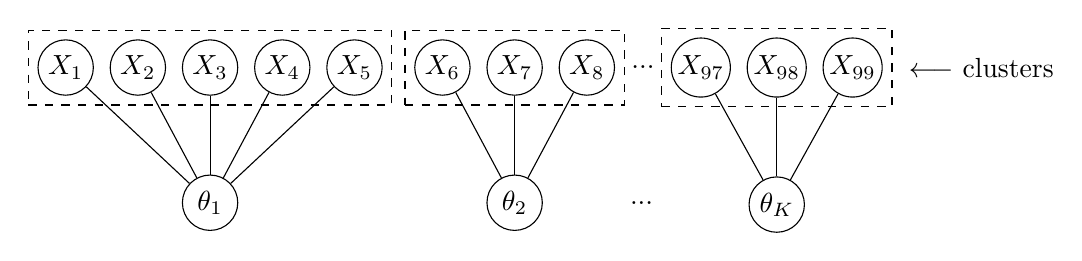
\begin{tikzpicture}[x=0.2cm]

  \FPeval{\spahalf}{clip(0.9)}
  \FPeval{\spamore}{clip(0.2)}

  \node[latent] (x-1)  {$X_1$} ;
  \foreach \i in {2,...,5}{
    \FPeval{\prev}{clip(\i - 1)}
    \node[latent, right=of x-\prev] (x-\i)  {$X_{\i}$} ;
  }
  \node[latent, right=of x-5, xshift=\spamore cm] (x-6)  {$X_6$} ;
  \foreach \i in {7,...,8}{
    \FPeval{\prev}{clip(\i - 1)}
    \node[latent, right=of x-\prev] (x-\i)  {$X_{\i}$} ;
  }
  \node[const, right=of x-8] (x-ellipsis)  {...} ;
  \node[latent, right=of x-ellipsis] (x-97)  {$X_{97}$} ;
  \node[latent, right=of x-97]       (x-98)  {$X_{98}$} ;
  \node[latent, right=of x-98]       (x-99)  {$X_{99}$} ;

  \gate {} {(x-1)(x-2)(x-3)(x-4)(x-5)} {}
  \gate {} {(x-6)(x-7)(x-8)} {}
  \gate {lastcluster} {(x-97)(x-98)(x-99)} {}
  \node[const, right=of lastcluster]    (cl-comment)  {$\longleftarrow$ clusters} ;

  \node[latent, below=of x-3]    (t-1)  {$\theta_{1}$} ;
  \foreach \i in {1,...,5}{
    \edge[-] {x-\i} {t-1}
  }
  \node[latent, below=of x-7]    (t-2)  {$\theta_{2}$} ;
  \foreach \i in {6,...,8}{
    \edge[-] {x-\i} {t-2}
  }
  \node[const, right=of t-2, xshift=\spahalf cm] (t-ellipsis)  {...} ;
  \node[latent, below=of x-98]    (t-k)  {$\theta_{K}$} ;
  \foreach \i in {97,...,99}{
    \edge[-] {x-\i} {t-k}
  }
  
\end{tikzpicture}

  \caption{Variable dependencies when learning one SVM per cluster (baseline used in Clustered SVM~\cite{gu2013clustered}).}
  \label{fig:gm-svmpercluster}
\end{figure}

\begin{figure}[h!]
  \centering
  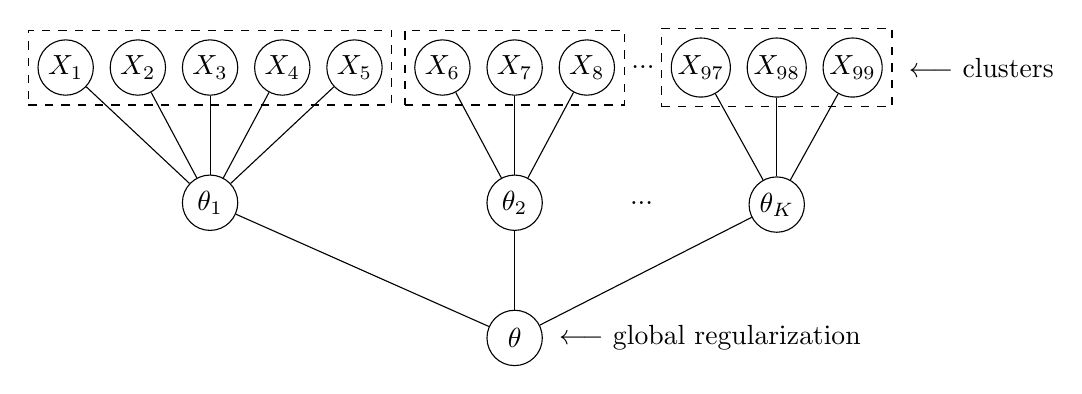
\begin{tikzpicture}[x=0.2cm]

  \FPeval{\spahalf}{clip(0.9)}
  \FPeval{\spamore}{clip(0.2)}

  \node[latent] (x-1)  {$X_1$} ;
  \foreach \i in {2,...,5}{
    \FPeval{\prev}{clip(\i - 1)}
    \node[latent, right=of x-\prev] (x-\i)  {$X_{\i}$} ;
  }
  \node[latent, right=of x-5, xshift=\spamore cm] (x-6)  {$X_6$} ;
  \foreach \i in {7,...,8}{
    \FPeval{\prev}{clip(\i - 1)}
    \node[latent, right=of x-\prev] (x-\i)  {$X_{\i}$} ;
  }
  \node[const, right=of x-8] (x-ellipsis)  {...} ;
  \node[latent, right=of x-ellipsis] (x-97)  {$X_{97}$} ;
  \node[latent, right=of x-97]       (x-98)  {$X_{98}$} ;
  \node[latent, right=of x-98]       (x-99)  {$X_{99}$} ;

  \gate {} {(x-1)(x-2)(x-3)(x-4)(x-5)} {}
  \gate {} {(x-6)(x-7)(x-8)} {}
  \gate {lastcluster} {(x-97)(x-98)(x-99)} {}
  \node[const, right=of lastcluster]    (cl-comment)  {$\longleftarrow$ clusters} ;

  \node[latent, below=of x-3]    (t-1)  {$\theta_{1}$} ;
  \foreach \i in {1,...,5}{
    \edge[-] {x-\i} {t-1}
  }
  \node[latent, below=of x-7]    (t-2)  {$\theta_{2}$} ;
  \foreach \i in {6,...,8}{
    \edge[-] {x-\i} {t-2}
  }
  \node[const, right=of t-2, xshift=\spahalf cm] (t-ellipsis)  {...} ;
  \node[latent, below=of x-98]    (t-k)  {$\theta_{K}$} ;
  \foreach \i in {97,...,99}{
    \edge[-] {x-\i} {t-k}
  }


  % addition to svmpercluster
  \node[latent, below=of t-2]    (t-global)  {$\theta$} ;
  \edge[-] {t-1,t-2,t-k} {t-global}
  \node[const, right=of t-global]    (t-global-comment)  {$\longleftarrow$ global regularization} ;
  
\end{tikzpicture}

  \caption{Variable dependencies for Clustered SVM~\cite{gu2013clustered}, where a common global regularization is used.}
  \label{fig:gm-clusteredsvm}
\end{figure}

\begin{figure}[h!]
  \centering
  
\newcommand{\mymul}[1]{{\mu}_{\mkern-0.66\thinmuskip\mathcal{L}, #1} }

\pgfdeclarelayer{bg}
\pgfsetlayers{bg,main}

\begin{tikzpicture}[x=0.2cm]

  \FPeval{\spahalf}{clip(0.9)}
  \FPeval{\spamore}{clip(0.2)}

  \node[latent] (x-1)  {$X_1$} ;
  \node[latent, below=of x-1] (mu-1)  {$\mymul{1}$} ;
  \foreach \i in {2,...,5}{
    \FPeval{\prev}{clip(\i - 1)}
    \node[latent, right=of x-\prev] (x-\i)  {$X_{\i}$} ;
    \node[latent, below=of x-\i] (mu-\i)  {$\mymul{\i}$} ;
  }
  \node[latent, right=of x-5, xshift=\spamore cm] (x-6)  {$X_6$} ;
  \node[latent, below=of x-6] (mu-6)  {$\mymul{6}$} ;
  \foreach \i in {7,...,8}{
    \FPeval{\prev}{clip(\i - 1)}
    \node[latent, right=of x-\prev] (x-\i)  {$X_{\i}$} ;
    \node[latent, below=of x-\i] (mu-\i)  {$\mymul{\i}$} ;
  }
  \node[const, right=of x-8] (x-ellipsis)  {...} ;
  \node[latent, right=of x-ellipsis] (x-97)  {$X_{97}$} ;
  \node[latent, right=of x-97]       (x-98)  {$X_{98}$} ;
  \node[latent, right=of x-98]       (x-99)  {$X_{99}$} ;
  \node[const, right=of mu-8] (mu-ellipsis)  {...} ;
  \node[latent, below=of x-97] (mu-97)  {$\mymul{97}$} ;
  \node[latent, below=of x-98] (mu-98)  {$\mymul{98}$} ;
  \node[latent, below=of x-99] (mu-99)  {$\mymul{99}$} ;
  \foreach \i in {1,...,8,97,98,99}{
    \edge[-] {x-\i} {mu-\i}
  }

  \gate {} {(x-1)(x-2)(x-3)(x-4)(x-5)} {}
  \gate {} {(x-6)(x-7)(x-8)} {}
  \gate {lastcluster} {(x-97)(x-98)(x-99)} {}
  \node[const, right=of lastcluster]    (cl-comment)  {$\longleftarrow$ clusters} ;

  
  % thetas
  \node[latent, below=of mu-3]    (t-1)  {$\theta_{1}$} ;
  \node[latent, below=of mu-7]    (t-2)  {$\theta_{2}$} ;
  \node[const, right=of t-2, xshift=\spahalf cm]   (t-ellipsis)  {...} ;
  \node[latent, below=of mu-98]    (t-k)  {$\theta_{K}$} ;
  \foreach \i in {1,...,5}{
    \edge[-] {mu-\i} {t-1}
  }
  \foreach \i in {6,...,8}{
    \edge[-] {mu-\i} {t-2}
  }
  \foreach \i in {97,...,99}{
    \edge[-] {mu-\i} {t-k}
  }

  % below
  \begin{pgfonlayer}{bg}
    \newcommand{\colorforb}{lightgray!75!blue}
    \newcommand{\colorforbb}{lightgray!75!green}
    \newcommand{\colorforL}{white!50!red}
    % b
    \node[latent, text=\colorforb, draw=\colorforb, below=of t-2, xshift=1.3cm]    (b)  {$\bm{b}$} ;
    \node[const, right=of b]    (b-comment)  {$\longleftarrow$ common bias} ;
    \foreach \i in {1,...,8,97,98,99}{
      \edge[-,color=\colorforb] {mu-\i} {b}
    }
    \edge[-,color=\colorforbb] {t-1} {b}
    \edge[-,color=\colorforbb] {t-2} {b}
    \edge[-,color=\colorforbb] {t-k} {b}
    % landmarks
    \node[latent, text=\colorforL, draw=\colorforL, right=of mu-99, xshift=0.5cm, yshift=-1.3cm] (L)  {$\bm{\mathcal{L}}$} ;
    %\edge[-,color=\colorforL] {mu-1} {L} % (no loop) good enough visually
    \foreach \i in {1,...,8,97,98,99}{
      \edge[-,color=\colorforL] {mu-\i} {L}
    }
    \node[const, right=of L]    (L-comment)  {$\longleftarrow$ landmarks} ;
  \end{pgfonlayer}

\end{tikzpicture}

  \caption{Variable dependencies for our model, \landSVM, where one SVM is learned per cluster but the local models interact through a common bias and $\mathcal{L}$, the set of landmarks.}
  \label{fig:gm-oursvm}
\end{figure}


\bibliographystyle{ieee}
\bibliography{paper}
\end{document}
